% !TEX root = Technologierecherche.tex
\section{Entladen}
\subsection{Kippen des Behälters}

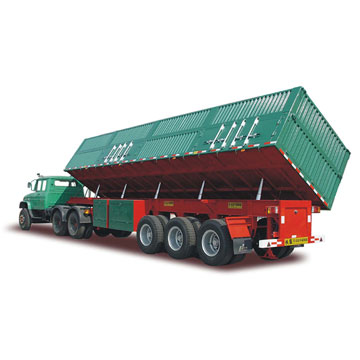
\includegraphics[width=0.5\textwidth]{Images/Entladen1.jpg}

Seitliches Entladen des Behälters

Vorteile:
\begin{itemize}
\item einfache Realisierung
\item wird in der Praxis angewandt
\end{itemize}

Nachteile:
\begin{itemize}
\item Nahes Heranfahren an Entladebehälter notwendig
\end{itemize}

\subsection{Seitliche Klappe öffnen}

Vorteil:
\begin{itemize}
\item sehr einfach realisierbar
\end{itemize}

\begin{flushleft}
Nachteile:
\end{flushleft}
\begin{itemize}
\item nicht automatisch wieder verschliessbar
\item fraglich ob Zielbereich einhaltbar ist
\end{itemize}

\subsection{Mit Greifer ausladen}

Vorteil:
\begin{itemize}
\item Greifer wird für 2 Funktion gebraucht (Einladen/Ausladen)
\end{itemize}

\begin{flushleft}
Nachteile:
\end{flushleft}
\begin{itemize}
\item schwierig gesamtes Schüttgut zu erwischen
\item aufwändiger Greifer
\item schwierig realisierbar
\end{itemize}